The following hyperparameters were used for all algorithms unless otherwise specified:
\begin{itemize}
    \item $\gamma = 0.95$
    \item $\theta = 10^{-16}$
    \item $\alpha = 0.1$
    \item $\epsilon = 0.1$
\end{itemize}

\subsection*{Policy Iteration}
\begin{figure}[ht]
\centering
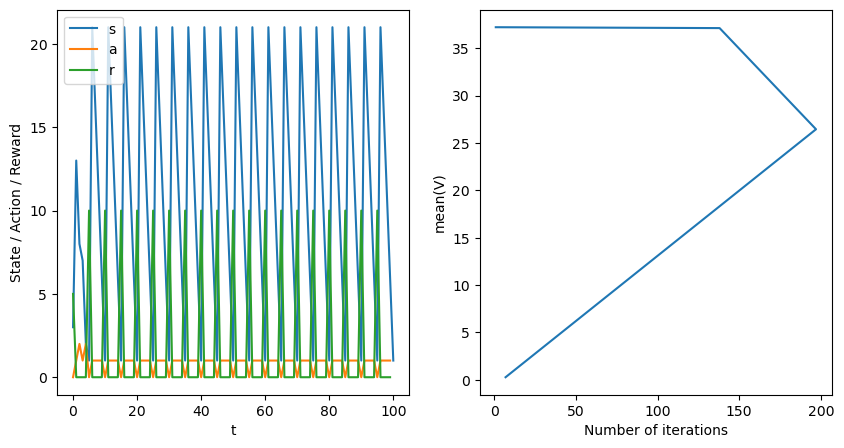
\includegraphics[width=0.8\linewidth]{gridworld/traj_return_policy_iteration.png}
\caption{Gridworld Trajectory and Learning Curve for Policy Iteration}
\label{fig:gridworld_traj_return_policy_iteration}
\end{figure}

\begin{figure}[ht]
\centering
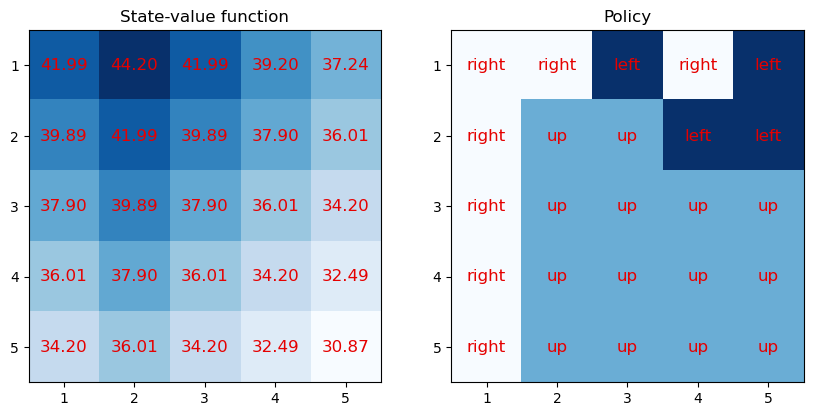
\includegraphics[width=0.8\linewidth]{gridworld/V_pi_policy_iteration.png}
\caption{Gridworld State Value Function and Policy for Policy Iteration}
\label{fig:gridworld_V_pi_policy_iteration}
\end{figure}

For the gridworld policy iteration, an example trajectory and learning curve are shown in Figure \ref{fig:gridworld_traj_return_policy_iteration}. The state value function and policy are shown in Figure \ref{fig:gridworld_V_pi_policy_iteration}. The policy iteration algorithm converges to the optimal policy in approximately 350 iterations.

\subsection*{Value Iteration}
\begin{figure}[ht]
\centering
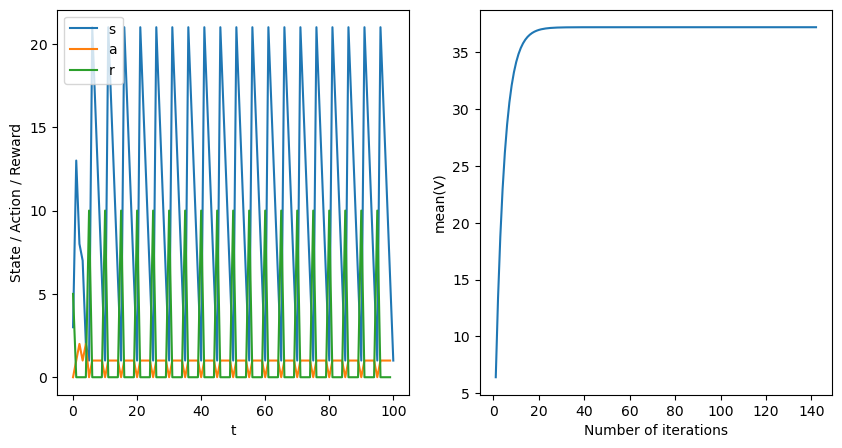
\includegraphics[width=0.8\linewidth]{gridworld/traj_return_value_iteration.png}
\caption{Gridworld Trajectory and Learning Curve for Value Iteration}
\label{fig:gridworld_traj_return_value_iteration}
\end{figure}

\begin{figure}[ht]
\centering
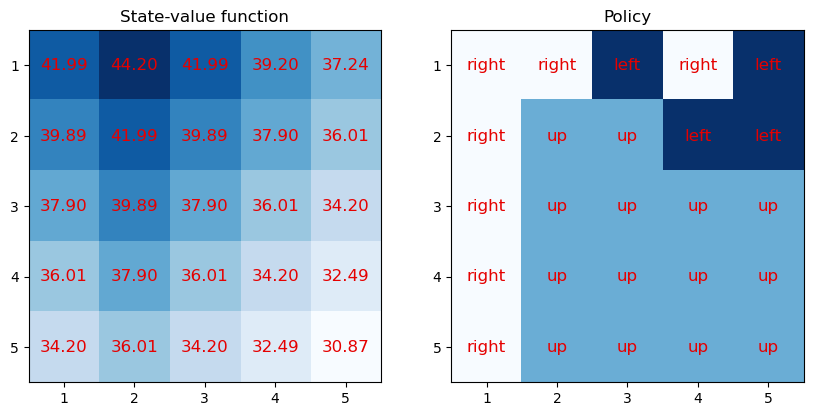
\includegraphics[width=0.8\linewidth]{gridworld/V_pi_value_iteration.png}
\caption{Gridworld State Value Function and Policy for Value Iteration}
\label{fig:gridworld_V_pi_value_iteration}
\end{figure}

For the gridworld value iteration, an example trajectory and learning curve are shown in Figure \ref{fig:gridworld_traj_return_value_iteration}. The state value function and policy are shown in Figure \ref{fig:gridworld_V_pi_value_iteration}. The value iteration algorithm converges to the optimal policy in approximately 140 iterations.

\subsection*{SARSA}
\begin{figure}[ht]
\centering
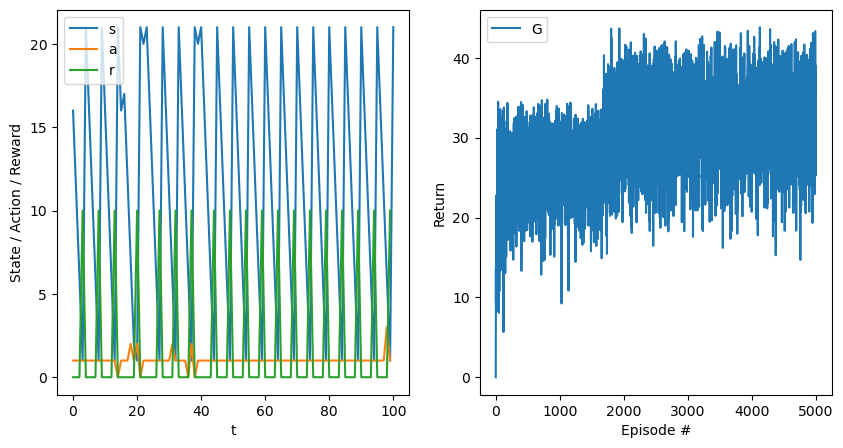
\includegraphics[width=0.8\linewidth]{gridworld/traj_return_sarsa.png}
\caption{Gridworld Trajectory and Learning Curve for SARSA}
\label{fig:gridworld_traj_return_sarsa}
\end{figure}

\begin{figure}[ht]
\centering
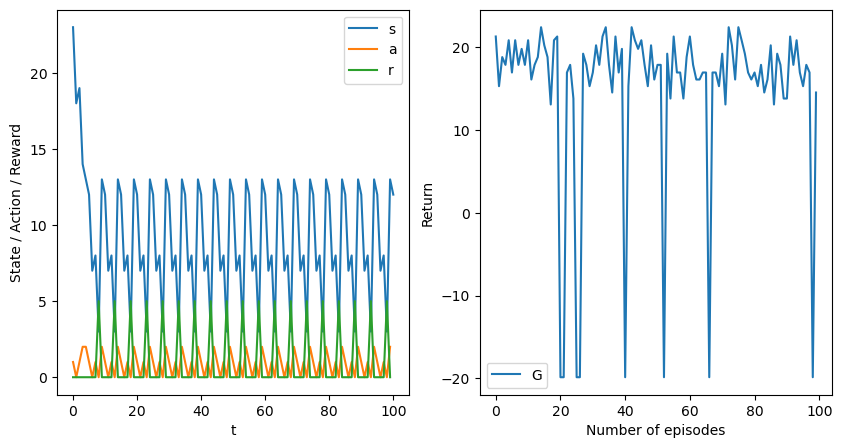
\includegraphics[width=0.8\linewidth]{gridworld/traj_return_td0_sarsa.png}
\caption{Gridworld Trajectory and Learning Curve for SARSA after TD(0)}
\label{fig:gridworld_traj_return_td0_sarsa}
\end{figure}

\begin{figure}[ht]
\centering
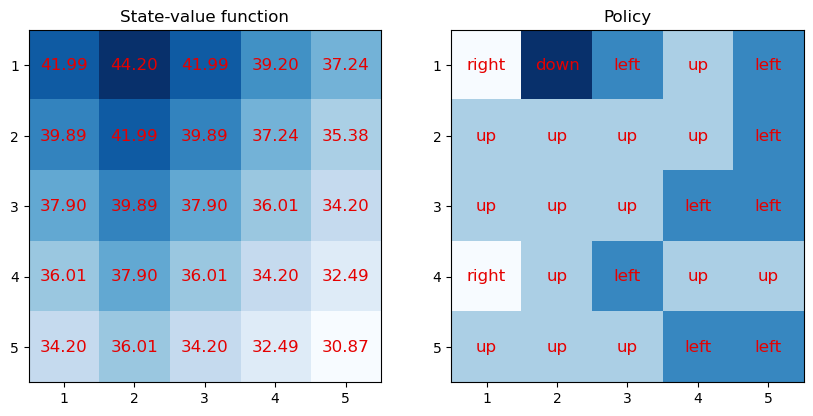
\includegraphics[width=0.8\linewidth]{gridworld/V_pi_sarsa.png}
\caption{Gridworld State Value Function and Policy for SARSA using TD(0)}
\label{fig:gridworld_V_pi_sarsa}
\end{figure}

\begin{figure}
\centering
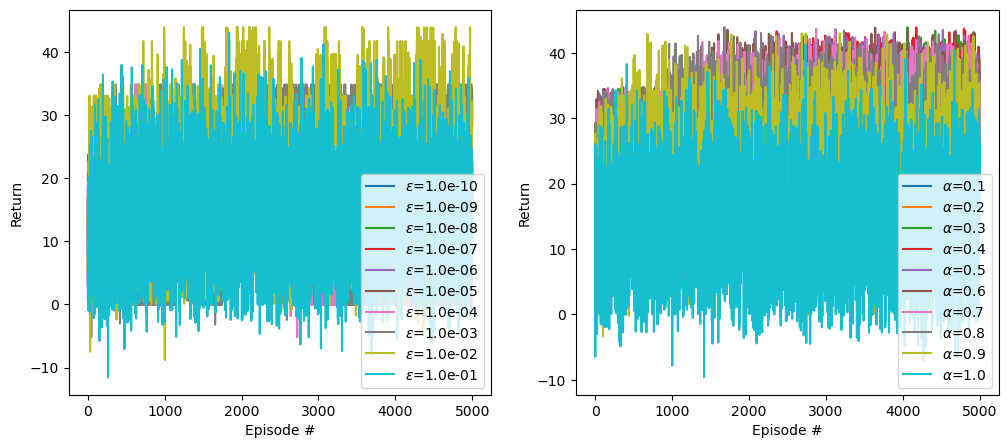
\includegraphics[width=0.8\linewidth]{gridworld/diff_epsilon_alpha_sarsa.png}
\caption{Gridworld Effect of $\epsilon$ and $\alpha$ on Learning Curve for SARSA}
\label{fig:gridworld_diff_epsilon_alpha_sarsa}
\end{figure}

For the gridworld SARSA algorithm, an example trajectory and learning curve are shown in Figure \ref{fig:gridworld_traj_return_sarsa}. The state value function and policy are shown in Figure \ref{fig:gridworld_V_pi_sarsa}. The SARSA algorithm shown here was run for 5000 episodes. Additionally, TD(0) was applied to the SARSA algorithm to derive a state value function. An example trajectory and learning curve are shown in Figure \ref{fig:gridworld_traj_return_td0_sarsa}. The state value function is nearly identical to the one generated by the value iteration and policy iteration algorithms. Additionally, the effect of varying $\epsilon$ and $\alpha$ on the learning curve is shown in Figure \ref{fig:gridworld_diff_epsilon_alpha_sarsa}.

\subsection*{Q-Learning}
\begin{figure}[ht]
\centering
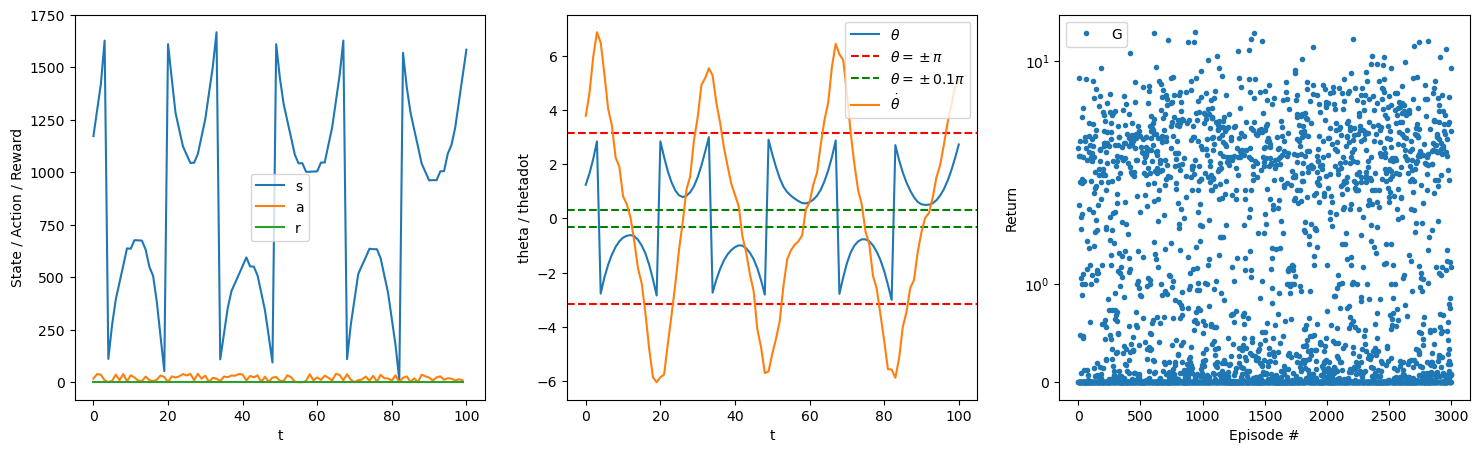
\includegraphics[width=0.8\linewidth]{gridworld/traj_return_q_learning.png}
\caption{Gridworld Trajectory and Learning Curve for Q-Learning}
\label{fig:gridworld_traj_return_q_learning}
\end{figure}

\begin{figure}[ht]
\centering
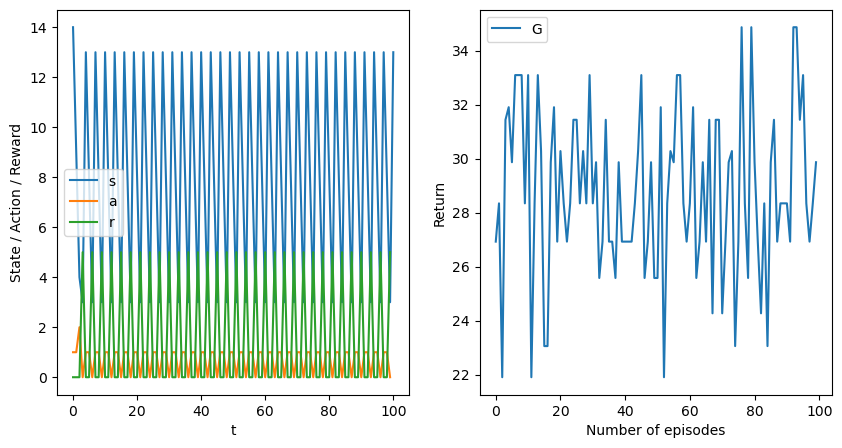
\includegraphics[width=0.8\linewidth]{gridworld/traj_return_td0_q_learning.png}
\caption{Gridworld Trajectory and Learning Curve for Q-Learning after TD(0)}
\label{fig:gridworld_traj_return_td0_q_learning}
\end{figure}

\begin{figure}[ht]
\centering
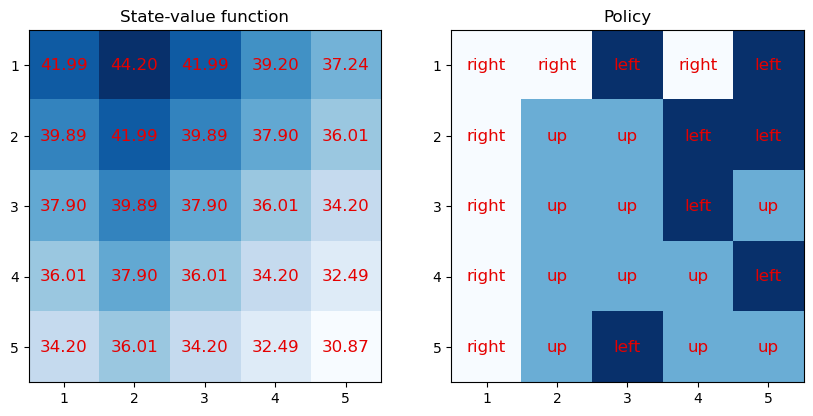
\includegraphics[width=0.8\linewidth]{gridworld/V_pi_q_learning.png}
\caption{Gridworld State Value Function and Policy for Q-Learning using TD(0)}
\label{fig:gridworld_V_pi_q_learning}
\end{figure}

\begin{figure}
\centering
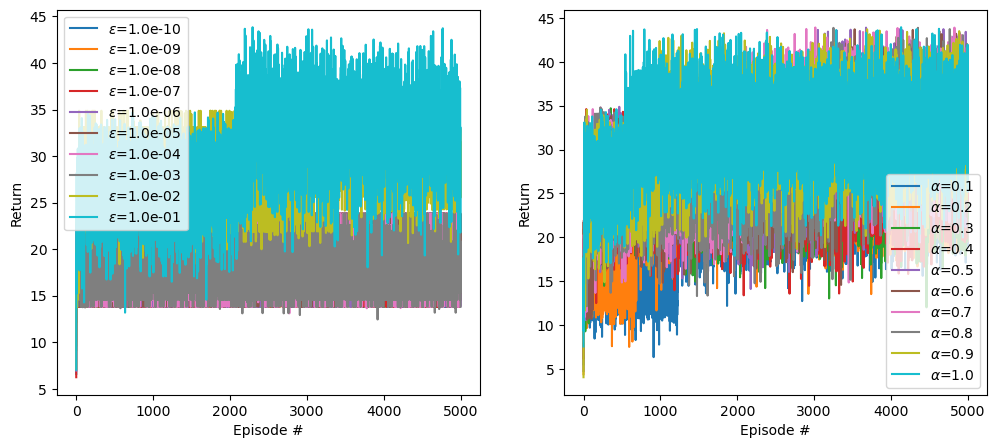
\includegraphics[width=0.8\linewidth]{gridworld/diff_epsilon_alpha_q_learning.png}
\caption{Gridworld Effect of $\epsilon$ and $\alpha$ on Learning Curve for Q-Learning}
\label{fig:gridworld_diff_epsilon_alpha_q_learning}
\end{figure}

For the gridworld Q-learning algorithm, an example trajectory and learning curve are shown in Figure \ref{fig:gridworld_traj_return_q_learning}. The state value function and policy are shown in Figure \ref{fig:gridworld_V_pi_q_learning}. The Q-learning algorithm shown here was run for 5000 episodes. Additionally, TD(0) was applied to the Q-learning algorithm to derive a state value function. An example trajectory and learning curve are shown in Figure \ref{fig:gridworld_traj_return_td0_q_learning}. The state value function is nearly identical to the one generated by the value iteration and policy iteration algorithms. Additionally, the effect of varying $\epsilon$ and $\alpha$ on the learning curve is shown in Figure \ref{fig:gridworld_diff_epsilon_alpha_q_learning}.

\FloatBarrier